%% DDR4 / DDR5 Timing Parameters — Full Glossary & Reference
%% Covers all symbols, full forms, formulae, and explanations
%% Author: Memory Controller Capstone Project

\documentclass[11pt,a4paper]{article}

%% ── Packages ────────────────────────────────────────────────────────────────
\usepackage[a4paper, top=22mm, bottom=22mm, left=22mm, right=22mm]{geometry}
\usepackage{fontenc}
\usepackage[T1]{fontenc}
\usepackage{lmodern}
\usepackage{microtype}
\usepackage{booktabs}
\usepackage{longtable}
\usepackage{array}
\usepackage{tabularx}
\usepackage{multirow}
\usepackage{xcolor}
\usepackage{colortbl}
\usepackage{amsmath}
\usepackage{amssymb}
\usepackage{enumitem}
\usepackage{fancyhdr}
\usepackage{titlesec}
\usepackage{parskip}
\usepackage{mdframed}
\usepackage{hyperref}
\usepackage{tikz}
\usepackage{pgfplots}
\pgfplotsset{compat=1.18}
\usetikzlibrary{arrows.meta, positioning, shapes.geometric, fit, backgrounds}

%% ── Colours ─────────────────────────────────────────────────────────────────
\definecolor{ddrblue}{RGB}{30, 90, 160}
\definecolor{ddrteal}{RGB}{0, 128, 128}
\definecolor{ddramber}{RGB}{200, 130, 0}
\definecolor{ddrgreen}{RGB}{0, 130, 80}
\definecolor{ddrred}{RGB}{180, 30, 30}
\definecolor{lightgray}{RGB}{245, 245, 245}
\definecolor{midgray}{RGB}{220, 220, 220}
\definecolor{rowblue}{RGB}{235, 243, 255}
\definecolor{rowgreen}{RGB}{235, 250, 240}
\definecolor{roworange}{RGB}{255, 245, 230}
\definecolor{rowred}{RGB}{255, 238, 238}
\definecolor{rowpurple}{RGB}{245, 235, 255}

%% ── Section formatting ───────────────────────────────────────────────────────
\titleformat{\section}{\large\bfseries\color{ddrblue}}{}{0em}{}[\titlerule]
\titleformat{\subsection}{\normalsize\bfseries\color{ddrteal}}{}{0em}{}
\titleformat{\subsubsection}{\normalsize\bfseries\color{ddramber}}{}{0em}{}

%% ── Header / Footer ─────────────────────────────────────────────────────────
\pagestyle{fancy}
\fancyhf{}
\renewcommand{\headrulewidth}{0.4pt}
\fancyhead[L]{\small\textcolor{ddrblue}{\textbf{DDR Timing Parameters Glossary}}}
\fancyhead[R]{\small\textcolor{gray}{JESD79-4 / JESD79-5}}
\fancyfoot[C]{\small\thepage}

%% ── Column types ─────────────────────────────────────────────────────────────
\newcolumntype{L}[1]{>{\raggedright\arraybackslash}p{#1}}
\newcolumntype{C}[1]{>{\centering\arraybackslash}p{#1}}
\newcolumntype{R}[1]{>{\raggedleft\arraybackslash}p{#1}}

%% ── Shorthand macros ─────────────────────────────────────────────────────────
\newcommand{\sym}[1]{\texttt{\textbf{#1}}}
\newcommand{\unit}[1]{\textit{#1}}
\newcommand{\formula}[1]{$#1$}
\newcommand{\ddr}[1]{\textcolor{ddrblue}{\textbf{#1}}}
\newcommand{\note}[1]{\textcolor{gray}{\small\textit{#1}}}

%% ── Framed note box ──────────────────────────────────────────────────────────
\newmdenv[
  backgroundcolor=rowblue,
  linecolor=ddrblue,
  linewidth=1pt,
  innerleftmargin=8pt,
  innerrightmargin=8pt,
  innertopmargin=6pt,
  innerbottommargin=6pt,
  roundcorner=4pt
]{notebox}

\newmdenv[
  backgroundcolor=roworange,
  linecolor=ddramber,
  linewidth=1pt,
  innerleftmargin=8pt,
  innerrightmargin=8pt,
  innertopmargin=6pt,
  innerbottommargin=6pt,
  roundcorner=4pt
]{warnbox}

%% ════════════════════════════════════════════════════════════════════════════
\begin{document}

\begin{titlepage}
  \centering
  \vspace*{2cm}
  {\Huge\bfseries\color{ddrblue} DDR Timing Parameters\\[0.4em]
  \Large Complete Glossary \& Reference Guide}\\[1.5em]
  {\large\color{ddrteal} DDR4 (JESD79-4) \quad\textbullet\quad DDR5 (JESD79-5)}\\[1em]
  {\normalsize Memory Controller Capstone Project}\\[0.5em]
  {\normalsize\color{gray} Covers all timing symbols, full forms, formulae, constraints, and inter-parameter relationships}
  \vfill
  \begin{tabular}{ll}
    \textbf{Standard} & JEDEC JESD79-4 (DDR4), JESD79-5 (DDR5) \\
    \textbf{Scope}     & MC Core Timing Reference \\
    \textbf{BL}        & BL8 (DDR4), BL16 (DDR5) \\
    \textbf{Corners}   & @200\,MHz (tCK=5\,ns) and @100\,MHz (tCK=10\,ns) \\
  \end{tabular}
  \vspace{2cm}
\end{titlepage}

\tableofcontents
\newpage

%% ════════════════════════════════════════════════════════════════════════════
\section{Notation and Conventions}

\begin{notebox}
\textbf{How to read timing values:} All timing constraints are expressed as a minimum number of clock cycles 
(\unit{nCK}) at the MC input clock. When a spec gives a value in nanoseconds, convert using
$n_{\text{CK}} = \lceil t_{\text{ns}} / t_{\text{CK}} \rceil$, subject to any stated minimum nCK floor.
\end{notebox}

\subsection{Key Abbreviations}

\begin{longtable}{L{2.4cm} L{4.5cm} L{8cm}}
\toprule
\textbf{Abbrev.} & \textbf{Full Form} & \textbf{Meaning} \\
\midrule
\endfirsthead
\toprule
\textbf{Abbrev.} & \textbf{Full Form} & \textbf{Meaning} \\
\midrule
\endhead
\bottomrule
\endfoot
nCK  & Number of Clocks & Integer clock cycle count at the DRAM/MC interface \\
ns   & Nanosecond       & Time unit; $1\,\text{ns} = 10^{-9}\,\text{s}$ \\
tCK  & Clock Period     & Reciprocal of clock frequency; tCK = 5\,ns @ 200\,MHz \\
BL   & Burst Length     & Number of data beats per read/write command. DDR4: BL8, DDR5: BL16 \\
BL/2 & Half Burst Length & Number of clock cycles the data bus is occupied. DDR4: 4, DDR5: 8 \\
CL   & CAS Latency      & Read latency from READ command to first data \\
CWL  & CAS Write Latency & Write latency from WRITE command to first data-in on DQ \\
AL   & Additive Latency  & Additional pipeline latency added to CL/CWL (usually 0) \\
RL   & Read Latency      & Total read latency = CL + AL \\
WL   & Write Latency     & Total write latency = CWL + AL \\
BG   & Bank Group        & Logical grouping of banks; DDR4: 4 BGs $\times$ 4 banks; DDR5: 2 BGs $\times$ 4 banks \\
AP   & Auto Precharge    & Automatic precharge at end of read/write burst \\
PDA  & Per-DRAM Addressability & DDR4/5 feature to address individual DRAM in a rank \\
DFI  & DRAM/PHY Interface & Standardised interface between MC and PHY \\
PHY  & Physical Layer    & Analogue I/O interface between chip and DRAM \\
DQ   & Data Bit          & Single data pin \\
DQS  & Data Strobe       & Differential strobe used for data capture \\
ODT  & On-Die Termination & Internal termination resistor in the DRAM \\
ZQ   & Impedance Calibration & Periodic calibration of output driver and ODT impedance \\
MRS/MRW & Mode Register Set/Write & Command to program DRAM mode registers \\
MPR  & Multi-Purpose Register & DDR4 special register for training patterns \\
MPC  & Multi-Purpose Command & DDR5 replacement for DDR4 MPC/ZQ mechanism \\
RFM  & Refresh Management & DDR5-only rowhammer mitigation; tracks row activations \\
RAA  & Row Activation Accumulator & DDR5 per-bank counter for RFM \\
ECS  & Error Check and Scrub & DDR5 inline ECC scrubbing mechanism \\
FGR  & Fine Granularity Refresh & Configurable tRFC modes (1x/2x/4x) \\
\end{longtable}

%% ════════════════════════════════════════════════════════════════════════════
\section{DRAM States}

A DRAM bank cycles through well-defined states. The memory controller must track
every bank's current state and issue commands only when the state and all timing
constraints are simultaneously satisfied.

\begin{center}
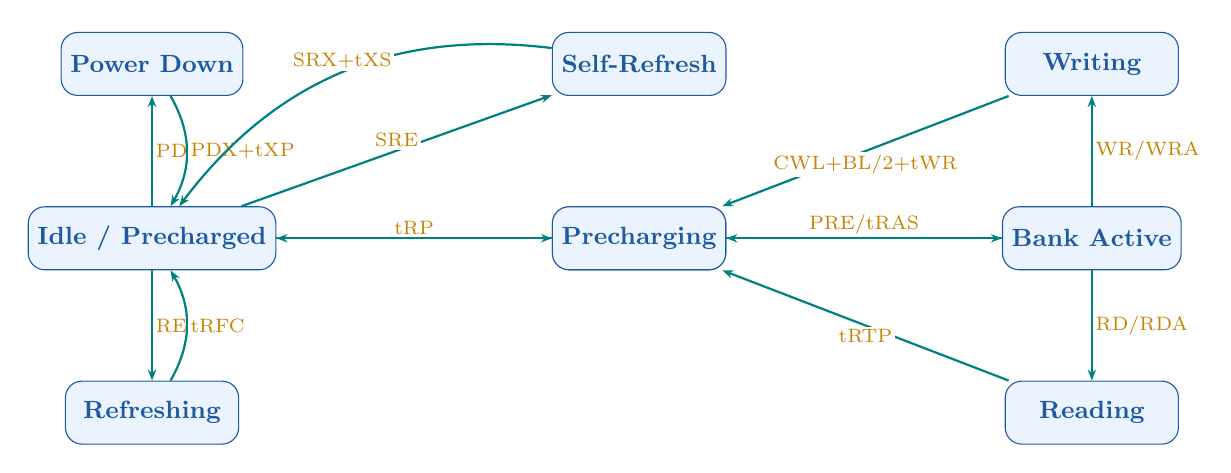
\begin{tikzpicture}[
  node distance=1.8cm and 2.4cm,
  state/.style={draw=ddrblue, fill=rowblue, rounded corners=6pt,
                minimum width=2.2cm, minimum height=0.8cm,
                font=\small\bfseries, text=ddrblue},
  arr/.style={-{Stealth[length=4pt]}, thick, color=ddrteal},
  lbl/.style={font=\scriptsize, color=ddramber, fill=white, inner sep=1pt}
]
  \node[state] (idle)    {Idle / Precharged};
  \node[state, right=3.5cm of idle]  (act)    {Activating};
  \node[state, right=3.5cm of act]   (active) {Bank Active};
  \node[state, below=1.4cm of active](rd)     {Reading};
  \node[state, above=1.4cm of active](wr)     {Writing};
  \node[state, left=3.5cm  of active](pre)    {Precharging};
  \node[state, below=1.4cm of idle]  (ref)    {Refreshing};
  \node[state, above=1.4cm of idle]  (pd)     {Power Down};
  \node[state, above=1.4cm of act]   (sr)     {Self-Refresh};

  \draw[arr] (idle)   -- node[lbl,above]{ACT}        (act);
  \draw[arr] (act)    -- node[lbl,above]{tRCD}        (active);
  \draw[arr] (active) -- node[lbl,right]{RD/RDA}      (rd);
  \draw[arr] (active) -- node[lbl,right]{WR/WRA}      (wr);
  \draw[arr] (active) -- node[lbl,above]{PRE/tRAS}    (pre);
  \draw[arr] (rd)     -- node[lbl,below]{tRTP}        (pre);
  \draw[arr] (wr)     -- node[lbl,below]{CWL+BL/2+tWR}(pre);
  \draw[arr] (pre)    -- node[lbl,above]{tRP}         (idle);
  \draw[arr] (idle)   -- node[lbl,right]{REF}         (ref);
  \draw[arr] (ref)    to[bend right=30] node[lbl,right]{tRFC}  (idle);
  \draw[arr] (idle)   -- node[lbl,right]{PDE}         (pd);
  \draw[arr] (pd)     to[bend left=30]  node[lbl,right]{PDX+tXP}(idle);
  \draw[arr] (idle)   -- node[lbl,above]{SRE}         (sr);
  \draw[arr] (sr)     to[bend right=30] node[lbl,above]{SRX+tXS}(idle);
\end{tikzpicture}
\end{center}

\vspace{0.5em}
\begin{warnbox}
\textbf{Controller responsibility:} The MC must maintain per-bank state and timer 
information for all 16 banks (DDR4: 4\,BG $\times$ 4) / (DDR5: 2\,BG $\times$ 4 sub-banks $\times$ 2\,BGs = 16 banks).
\end{warnbox}

%% ════════════════════════════════════════════════════════════════════════════
\section{Activation and Precharge Timing}

These parameters govern how long a row stays open and the overhead of opening/closing it.

\begin{longtable}{L{2.2cm} L{4.8cm} L{3.5cm} L{4cm}}
\toprule
\textbf{Symbol} & \textbf{Full Form} & \textbf{Typical Value} & \textbf{Explanation} \\
\midrule
\endfirsthead
\toprule
\textbf{Symbol} & \textbf{Full Form} & \textbf{Typical Value} & \textbf{Explanation} \\
\midrule
\endhead
\bottomrule
\endfoot

\rowcolor{rowblue}
\sym{tRCD} & RAS-to-CAS Delay & DDR4: 12.5\,ns (4\,nCK @200)\newline DDR5: 18\,ns (4\,nCK @200) &
  Minimum time from ACT command to first READ or WRITE command on the same bank. 
  Represents the time for the sense amplifiers to latch the row data after activation. \\

\sym{tRP} & Row Precharge Time & DDR4: 12.5\,ns (4\,nCK)\newline DDR5: 18\,ns (4\,nCK) &
  Minimum time from PRE command until the bank is ready to be activated again.
  The bitlines must be equalised and the row must return to idle before a new ACT. \\

\rowcolor{rowblue}
\sym{tRAS} & Row Active Time (min) & DDR4: 35\,ns (7\,nCK)\newline DDR5: 32\,ns (7\,nCK) &
  Minimum time a row must stay activated after ACT before a PRE command may be issued.
  This ensures the sense amplifiers have fully restored the cell charge.
  $\text{tRAS(min)} \leq t_{\text{ACT}} \leq \text{tRAS(max)}$. \\

\sym{tRAS\,(max)} & Row Active Time (max) & $9 \times \text{tREFI}$ &
  Maximum time a row may remain open without a precharge. If exceeded, refresh cannot
  be serviced correctly. The MC must precharge within this window. \\

\rowcolor{rowblue}
\sym{tRC} & Row Cycle Time & DDR4: 47.5\,ns \newline DDR5: 50\,ns &
  Minimum time from one ACT to the next ACT on the \textit{same} bank.
  $\text{tRC} = \text{tRAS} + \text{tRP}$. Prevents consecutive activations before bitline recovery. \\

\sym{tRTP} & Internal Read-to-Precharge & \texttt{max(4\,nCK, 7.5\,ns)} &
  Minimum delay from a READ command to a PRE on the same bank.
  The internal sense-amplifier must complete the column read before precharging can begin.
  For reads with auto-precharge (RDA), hidden precharge starts at RD+tRTP internally. \\

\rowcolor{rowblue}
\sym{tWR} & Write Recovery Time & DDR4: 15\,ns \newline DDR5: 30\,ns &
  Minimum time from the last write data burst until a PRE command may be issued to the same bank.
  The write data must be fully restored in the DRAM cells before precharge.
  $\text{WR-to-PRE} = \text{CWL} + \text{BL/2} + \text{tWR}$. \\

\sym{tDAL} & Write-to-ACT Delay (Auto Precharge) & $\text{tWR} + \text{tRP}$ &
  For write-with-auto-precharge (WRA), the time from the WRA command until a new ACT can be issued 
  to the same bank. $\text{tDAL} = \text{tWR} + \text{tRP}$. \\

\rowcolor{rowblue}
\sym{tRRD\_L} & ACT-to-ACT Delay (Same Bank Group) & \texttt{max(4\,nCK, 4.9--7.5\,ns)} &
  Minimum time between two successive ACT commands targeting the \textit{same} bank group.
  Higher than tRRD\_S because same-BG activations share internal sensing resources. \\

\sym{tRRD\_S} & ACT-to-ACT Delay (Different Bank Group) & \texttt{max(4\,nCK, 2.5--5\,ns)} &
  Minimum time between two successive ACT commands in \textit{different} bank groups.
  Relaxed compared to tRRD\_L since inter-BG resource conflicts are minimal. \\

\rowcolor{rowblue}
\sym{tFAW} & Four-Activate Window & DDR4: 35\,ns \newline DDR5: 10\,ns (tFAW) &
  A rolling time window in which no more than four ACT commands may be issued across all banks.
  This limits peak power consumption during multiple simultaneous row activations.
  The MC must maintain a sliding window counter of the last 4 ACT timestamps. \\

\sym{tPPD} & PRE-to-PRE Delay & 2\,nCK &
  Minimum time between any two precharge commands (PRE or PREA), regardless of bank.
  Prevents command bus contention on back-to-back precharge operations. \\
\end{longtable}

%% ════════════════════════════════════════════════════════════════════════════
\section{Read and Write Data Timing}

\begin{longtable}{L{2.2cm} L{4.8cm} L{3.5cm} L{4cm}}
\toprule
\textbf{Symbol} & \textbf{Full Form} & \textbf{Typical Value} & \textbf{Explanation} \\
\midrule
\endfirsthead
\toprule
\textbf{Symbol} & \textbf{Full Form} & \textbf{Typical Value} & \textbf{Explanation} \\
\midrule
\endhead
\bottomrule
\endfoot

\rowcolor{rowgreen}
\sym{CL} & CAS Latency & DDR4: 9--22\,nCK\newline DDR5: 22--52\,nCK &
  Number of clock cycles from a READ command to the first data appearing on DQ.
  Higher clock frequencies require higher CL values (same ns delay). \\

\sym{CWL} & CAS Write Latency & DDR4: 9--18\,nCK \newline DDR5: CL$-$2 &
  Number of clock cycles from a WRITE command to the first data-in on DQ.
  Always $\leq$ CL. In DDR5, CWL = CL$-$2 per spec Table~9. \\

\rowcolor{rowgreen}
\sym{AL} & Additive Latency & 0, CL$-$1, or CL$-$2 &
  Extra pipeline latency added before the effective CAS operation.
  Increases RL/WL without changing the physical CL, useful for command bus scheduling.
  $\text{RL} = \text{CL} + \text{AL}$;\ $\text{WL} = \text{CWL} + \text{AL}$. \\

\sym{RL} & Read Latency & = CL + AL &
  Total number of clock cycles from a READ command to first valid DQ data.
  Used in read-to-write turnaround formula: $\text{RTW} = \text{RL} + \text{BL/2} - \text{WL} + 2$. \\

\rowcolor{rowgreen}
\sym{WL} & Write Latency & = CWL + AL &
  Total number of clock cycles from a WRITE command to first DQ data driven by the controller.
  Governs write-to-read turnaround: $\text{WTR} = \text{WL} + \text{BL/2} + \text{tWTR}$. \\

\sym{tCCD\_L} & CAS-to-CAS Delay (Same Bank Group, Long) & DDR4: 5--8\,nCK\newline DDR5: 8\,nCK &
  Minimum time between two consecutive READ or WRITE commands targeting the \textit{same} bank group.
  Longer than tCCD\_S because same-BG data path resources (sense amps, I/O gating) are shared. \\

\rowcolor{rowgreen}
\sym{tCCD\_S} & CAS-to-CAS Delay (Different Bank Group, Short) & DDR4: 4\,nCK\newline DDR5: BL/2 = 8\,nCK &
  Minimum time between two consecutive READ or WRITE commands in \textit{different} bank groups.
  In DDR5 this equals BL/2 because the data bus is always occupied for exactly BL/2 cycles. \\

\sym{tWTR\_L} & Write-to-Read Turnaround (Same Bank Group) & \texttt{max(4\,nCK, 7.5\,ns)} &
  After the last write data clock, the minimum number of cycles before a READ command
  can be issued in the \textit{same} bank group. Guards DQ bus ownership transfer.
  Formula: $\text{WTR\_cmd} = \text{WL} + \text{BL/2} + \text{tWTR\_L}$. \\

\rowcolor{rowgreen}
\sym{tWTR\_S} & Write-to-Read Turnaround (Different Bank Group) & \texttt{max(2\,nCK, 2.5\,ns)} &
  Same as tWTR\_L but for different bank groups, where bus contention resolves faster.
  Formula: $\text{WTR\_cmd} = \text{WL} + \text{BL/2} + \text{tWTR\_S}$. \\

\sym{tRTW} & Read-to-Write Turnaround & \multicolumn{1}{l}{DDR4: $\text{RL}+\frac{\text{BL}}{2}-\text{WL}+2$} &
  Minimum time from a READ command before a WRITE command may follow, ensuring the
  read DQS postamble does not clash with the write preamble.
  In DDR4 with 1tCK write preamble: $+2$; with 2tCK preamble: $+3$. \\

\rowcolor{rowgreen}
\sym{tBURST} & Burst Duration & BL/2 clock cycles &
  Time the DQ data bus is occupied for one READ or WRITE operation.
  DDR4: 4 clock cycles (BL8); DDR5: 8 clock cycles (BL16). \\

\sym{tWPRE} & Write Preamble & 1\,tCK or 2\,tCK &
  The DQS high-Z$\rightarrow$low transition before first write data strobe.
  Default is 1tCK; 2tCK mode is available for higher frequencies (MR4 in DDR4, MR8 in DDR5). \\

\rowcolor{rowgreen}
\sym{tRPRE} & Read Preamble & 1\,tCK or 2\,tCK &
  The DQS idle-to-active transition window before first read data strobe.
  2tCK preamble improves setup margin at higher speeds. \\

\sym{tRPST} & Read Postamble & 0.5\,tCK &
  Minimum DQS active time after the last read data strobe before DQS returns to high-Z. \\

\rowcolor{rowgreen}
\sym{tWPST} & Write Postamble & 0.5\,tCK &
  Minimum DQS active time after the last write data strobe. \\
\end{longtable}

%% ════════════════════════════════════════════════════════════════════════════
\section{Refresh Timing}

Refresh is mandatory to prevent data loss. DDR4 and DDR5 differ significantly 
in refresh granularity and rowhammer management.

\begin{longtable}{L{2.2cm} L{4.8cm} L{3.5cm} L{4cm}}
\toprule
\textbf{Symbol} & \textbf{Full Form} & \textbf{Typical Value} & \textbf{Explanation} \\
\midrule
\endfirsthead
\toprule
\textbf{Symbol} & \textbf{Full Form} & \textbf{Typical Value} & \textbf{Explanation} \\
\midrule
\endhead
\bottomrule
\endfoot

\rowcolor{roworange}
\sym{tREFI} & Average Refresh Interval & DDR4: 7.8\,µs\newline DDR5: 3.9\,µs &
  Average time between consecutive REFRESH commands at normal temperature ($\leq$85°C).
  The MC must issue a REF command at least every tREFI on average.
  Up to $8\times$ postponement is allowed (up to $9\times$ tREFI total). \\

\sym{tRFC1} & Refresh Cycle Time (Normal mode, 1x) & DDR4/8Gb: 350\,ns\newline DDR5/8Gb: 195\,ns &
  Minimum time the DRAM requires after a REFRESH (REFab) command before any other command.
  All banks are unavailable during this period. Smaller devices have shorter tRFC1. \\

\rowcolor{roworange}
\sym{tRFC2} & Refresh Cycle Time (Fine Granularity 2x) & DDR4/8Gb: 260\,ns\newline DDR5: N/A &
  Used in DDR4 Fine Granularity Refresh (FGR) 2x mode where REF is issued at $2\times$ normal rate.
  Each refresh is shorter, reducing latency impact per REF but doubling REF frequency. \\

\sym{tRFC4} & Refresh Cycle Time (Fine Granularity 4x) & DDR4/8Gb: 160\,ns &
  Used in DDR4 FGR 4x mode (quadruple refresh rate). 
  Shortest tRFC; used in tXS\_FAST path for rapid SR exit. \\

\rowcolor{roworange}
\sym{tRFCsb} & Refresh Cycle Time (Same-Bank, DDR5) & DDR5: $\sim$115\,ns (8Gb) &
  \textbf{DDR5 only.} Time required after a same-bank refresh (REFsb) command.
  Only one bank is refreshed, so all other banks remain accessible, increasing effective bandwidth. \\

\sym{tXS} & Exit Self-Refresh to Normal (no DLL lock) & tRFC1 + 10\,ns &
  Minimum time after Self-Refresh Exit (SRX) before any command not requiring a locked DLL.
  $\text{tXS} = \text{tRFC1(min)} + 10\,\text{ns}$. \\

\rowcolor{roworange}
\sym{tXS\_FAST} & Exit SR to MRS/ZQCL (DDR4) & tRFC4 + 10\,ns &
  \textbf{DDR4 only.} A fast SRX path allowing Mode Register Set and ZQCL commands
  before tXS expires, using the shorter tRFC4 base. \\

\sym{tXS\_ABORT} & Exit SR-Abort to Commands & tRFC4 + 10\,ns &
  \textbf{DDR4 only.} When self-refresh is aborted (CKE raised while SR entry in progress),
  a shorter wait applies before commands are legal. \\

\rowcolor{roworange}
\sym{tXSDLL} & Exit SR to Commands Requiring DLL Lock & tDLLK &
  After SRX, commands like READ that need a locked DLL must wait until tDLLK cycles
  after a DLL Reset MRS before they are reliable. \\

\end{longtable}

\subsection{DDR5-Only Refresh Terms}

\begin{longtable}{L{2.2cm} L{4.8cm} L{3cm} L{5cm}}
\toprule
\textbf{Symbol} & \textbf{Full Form} & \textbf{Value} & \textbf{Explanation} \\
\midrule
\endfirsthead
\toprule
\textbf{Symbol} & \textbf{Full Form} & \textbf{Value} & \textbf{Explanation} \\
\midrule
\endhead
\bottomrule
\endfoot

\rowcolor{roworange}
\sym{REFab} & All-Bank Refresh & Command & Refreshes all banks simultaneously. 
  Equivalent to DDR4 REF. All 16 banks are unavailable for tRFC1 duration. \\

\sym{REFsb} & Same-Bank Refresh & Command & \textbf{DDR5 only.} Refreshes a single bank.
  Other banks remain accessible. tRFCsb $\ll$ tRFC1. Enables higher REF throughput. \\

\rowcolor{roworange}
\sym{RFM} & Refresh Management Command & Command & \textbf{DDR5 only.} Issued when per-bank RAA 
  counter reaches RAAIMT threshold. Adds one extra targeted refresh to mitigate rowhammer. \\

\sym{RAA} & Row Activation Accumulator & Counter (per bank) & Per-bank counter in DDR5 that 
  increments on each ACT and decrements by RAADec on each REF. 
  When RAA $\leq$ RAAIMT the MC must issue an RFM command. \\

\rowcolor{roworange}
\sym{RAAIMT} & RAA Initial Management Threshold & MR configurable & The RAA value at which 
  the MC \textit{must} issue an RFM. Typically set to half the rowhammer threshold. \\

\sym{RAAMMT} & RAA Maximum Management Threshold & MR configurable & The RAA value above which 
  DRAM may disable internal rowhammer management. Always $\geq$ RAAIMT. \\

\rowcolor{roworange}
\sym{tRFM} & Refresh Management Cycle Time & $\sim$195\,ns (same as tRFC1) & 
  Time the DRAM requires after an RFM command before the next command on that bank. \\

\sym{ECS} & Error Check and Scrub & Feature & DDR5 inline ECC: the DRAM scrubs its
  own ECC during refresh windows. Controlled by MR14/MR15. tECS governs scrub window. \\
\end{longtable}

%% ════════════════════════════════════════════════════════════════════════════
\section{Power Down and Self-Refresh Timing}

\begin{longtable}{L{2.2cm} L{4.8cm} L{3.5cm} L{4cm}}
\toprule
\textbf{Symbol} & \textbf{Full Form} & \textbf{Typical Value} & \textbf{Explanation} \\
\midrule
\endfirsthead
\toprule
\textbf{Symbol} & \textbf{Full Form} & \textbf{Typical Value} & \textbf{Explanation} \\
\midrule
\endhead
\bottomrule
\endfoot

\rowcolor{rowpurple}
\sym{tXP} & Exit Power Down to Command & \texttt{max(4\,nCK, 6\,ns)} &
  Minimum time from Power-Down Exit (PDX, i.e., CKE rising) until a valid command may be issued.
  During power down, ODT and DLL may be in reduced states that need recovery time. \\

\sym{tCKE} & CKE Minimum Pulse Width & \texttt{max(3\,nCK, 5\,ns)} &
  Minimum time CKE must be held LOW (for power down) or HIGH (in normal operation).
  Guards against glitches on the CKE pin. \\

\rowcolor{rowpurple}
\sym{tCKSRE} & Valid Clock Requirement after SRE/PDE & \texttt{max(5\,nCK, 10\,ns)} &
  After CKE is deasserted for Self-Refresh Entry (SRE) or Power-Down Entry (PDE),
  the clock must remain stable and valid for at least tCKSRE before being stopped (SRE) 
  or left running (PDE). Ensures proper internal latching of the mode change. \\

\sym{tCKSRX} & Valid Clock Requirement before SRX/PDX & \texttt{max(5\,nCK, 10\,ns)} &
  Before asserting CKE for Self-Refresh Exit (SRX) or Power-Down Exit (PDX),
  the clock must be stable for at least tCKSRX. 
  Ensures the DRAM PLL/DLL has a clean reference before exit. \\

\rowcolor{rowpurple}
\sym{tCKESR} & Min CKE Low Width in Self-Refresh & tCKE + 1\,nCK &
  Minimum time CKE must remain LOW during self-refresh before it can be raised for SRX.
  $\text{tCKESR} = \text{tCKE(min)} + 1\,\text{nCK}$. \\

\sym{tXPR} & Exit Reset to First MRS Command & \texttt{max(5\,nCK, tRFC1+10\,ns)} &
  After power-up reset, minimum delay before the first MRS command.
  This is the same as tXS since the DRAM runs its internal initialisation like a SR exit. \\

\rowcolor{rowpurple}
\sym{tACTPDEN} & ACT to Power-Down Entry & 1\,nCK (DDR4-1600)\newline 2\,nCK (DDR4-2400+) &
  Minimum time between an ACT command and CKE deassert for power-down entry.
  Ensures ACT is properly latched before CKE falls. \\

\sym{tRDPDEN} & Read to Power-Down Entry & $\text{RL} + \text{BL/2} + 1$ &
  Minimum delay from READ command until CKE may fall for power-down.
  Ensures all read data has been driven out before the DRAM powers down its output drivers. \\

\rowcolor{rowpurple}
\sym{tWRPDEN} & Write to Power-Down Entry (BL8/OTF) & $\text{WL} + \text{BL/2} + \text{tWR(nCK)}$ &
  Minimum delay from WRITE command until CKE may fall.
  Write data must be fully written to the DRAM array before power down. \\

\sym{tWRAPDEN} & Write-with-AP to Power-Down Entry & $\text{WL} + \text{BL/2} + \text{WR} + 1$ &
  Similar to tWRPDEN but adds 1 extra cycle for the auto-precharge internal operation. \\

\rowcolor{rowpurple}
\sym{tREFPDEN} & REF to Power-Down Entry & 1--2\,nCK &
  Minimum delay from REFRESH command until power-down may be entered.
  The REF command must be latched before CKE falls. \\

\sym{tMRSPDEN} & MRS to Power-Down Entry & tMOD (min) &
  After a Mode Register Set, the DRAM must have tMOD before power-down may be entered.
  Mode register update must complete before the DRAM powers down its logic. \\

\rowcolor{rowpurple}
\sym{tPD\,(max)} & Maximum Power-Down Duration & $9 \times \text{tREFI}$ &
  The DRAM may remain in power-down for at most $9 \times \text{tREFI}$ without losing data.
  The MC must track power-down entry time and schedule exit before this limit. \\

\sym{MPSM} & Maximum Power Saving Mode & Mode &
  \textbf{DDR4/5.} A deeper power state beyond normal power-down. The clock may also stop.
  Exit requires additional recovery time (tXMP/tXMPDLL). \\
\end{longtable}

%% ════════════════════════════════════════════════════════════════════════════
\section{Mode Register Set Timing}

\begin{longtable}{L{2.2cm} L{4.8cm} L{3.5cm} L{4cm}}
\toprule
\textbf{Symbol} & \textbf{Full Form} & \textbf{Typical Value} & \textbf{Explanation} \\
\midrule
\endfirsthead
\toprule
\textbf{Symbol} & \textbf{Full Form} & \textbf{Typical Value} & \textbf{Explanation} \\
\midrule
\endhead
\bottomrule
\endfoot

\rowcolor{rowred}
\sym{tMRD} & Mode Register Set Command Period & DDR4: 8\,nCK\newline DDR5: 16\,nCK &
  Minimum time between two consecutive MRS/MRW commands.
  Allows the DRAM's internal mode register update logic to settle between writes. \\

\sym{tMOD} & Mode Register Set Update Delay & DDR4: \texttt{max(24\,nCK, 15\,ns)}\newline DDR5: N/A (uses tMRD) &
  \textbf{DDR4 only.} Minimum delay from the last MRS command to the first \textit{non-MRS} command.
  The DRAM needs tMOD to propagate new register settings into the datapath (CL, CWL, etc.).
  tMRD governs MRS-to-MRS spacing; tMOD governs MRS-to-any-other spacing. \\

\rowcolor{rowred}
\sym{tMOD (DDR5)} & Mode Register Update Delay & DDR5: Not separately defined & 
  In DDR5, MRW (Mode Register Write) timing is governed by tMRD only.
  tMOD-style behaviour is absorbed into the DFI/PHY command scheduling. \\

\sym{tMPRR} & MPR Recovery Time & 1\,nCK &
  \textbf{DDR4 only.} Minimum time after MPR read/write before the next command. \\

\rowcolor{rowred}
\sym{tWR\_MPR} & MPR Write Recovery & tMOD(min) &
  \textbf{DDR4 only.} After an MRS that modifies the MPR register, tMOD must pass
  before another command (effectively tMOD clears any MPR state). \\
\end{longtable}

%% ════════════════════════════════════════════════════════════════════════════
\section{ZQ Calibration Timing}

ZQ calibration compensates for process, voltage, and temperature (PVT) drift in
the output driver and ODT impedance. The DRAM calibrates itself using an external
precision resistor on the ZQ pin.

\begin{longtable}{L{2.2cm} L{4.8cm} L{3.5cm} L{4cm}}
\toprule
\textbf{Symbol} & \textbf{Full Form} & \textbf{Typical Value} & \textbf{Explanation} \\
\midrule
\endfirsthead
\toprule
\textbf{Symbol} & \textbf{Full Form} & \textbf{Typical Value} & \textbf{Explanation} \\
\midrule
\endhead
\bottomrule
\endfoot

\rowcolor{rowgreen}
\sym{tZQinit} & ZQ Initial Calibration Time & 1024\,nCK &
  Time required for power-up ZQ long calibration (ZQCL).
  Issued once during initialisation after all MRS commands are loaded.
  The DRAM is unavailable for any other command during tZQinit. \\

\sym{tZQoper} & ZQ Long Calibration Time (Normal) & 512\,nCK &
  Time for a periodic ZQCL command during normal operation (e.g., temperature change).
  Shorter than tZQinit as the initial calibration has already run. \\

\rowcolor{rowgreen}
\sym{tZQCS} & ZQ Short Calibration Time & 128\,nCK &
  Time for a ZQCS (short calibration) command, used for periodic fine-tuning.
  Less accurate than ZQCL but much faster; typically issued every $\sim$128\,µs. \\

\sym{tZQCAL} & ZQ Calibration Start Duration (DDR5) & DDR5: 1\,µs (MPC: ZQCAL Start) &
  \textbf{DDR5 only.} DDR5 uses MPC commands (MPC ZQCAL Start $\rightarrow$ wait tZQCAL 
  $\rightarrow$ MPC ZQCAL Latch) instead of ZQCL/ZQCS. \\

\rowcolor{rowgreen}
\sym{tZQLAT} & ZQ Latch Time (DDR5) & DDR5: 30\,nCK &
  \textbf{DDR5 only.} Time after the MPC ZQCAL Latch command before the DRAM can accept
  other commands. Allows the calibration result to propagate to the output drivers. \\
\end{longtable}

%% ════════════════════════════════════════════════════════════════════════════
\section{DLL and Clock Timing}

\begin{longtable}{L{2.2cm} L{4.8cm} L{3.5cm} L{4cm}}
\toprule
\textbf{Symbol} & \textbf{Full Form} & \textbf{Typical Value} & \textbf{Explanation} \\
\midrule
\endfirsthead
\toprule
\textbf{Symbol} & \textbf{Full Form} & \textbf{Typical Value} & \textbf{Explanation} \\
\midrule
\endhead
\bottomrule
\endfoot

\rowcolor{rowblue}
\sym{tDLLK} & DLL Lock Time & DDR4: 512--1024\,nCK\newline DDR5: 1024\,nCK &
  After a DLL Reset MRS command, the DLL requires tDLLK clock cycles to re-lock.
  Commands requiring a locked DLL (primarily READ) are illegal until tDLLK expires.
  The MC must insert NOPs/DES during this window. \\

\sym{tCK(avg)} & Average Clock Cycle Time & Reciprocal of data rate / 2 &
  The average period of the input clock over many cycles.
  Defines the operating frequency and hence all nCK-based timing values. \\

\rowcolor{rowblue}
\sym{tCH(avg)} & Average Clock High Pulse Width & 0.48--0.52 $\times$ tCK &
  The high pulse of the differential clock (CK\_t high, CK\_c low) must occupy 
  48--52\% of each clock period for reliable sampling. \\

\sym{tCL(avg)} & Average Clock Low Pulse Width & 0.48--0.52 $\times$ tCK &
  Complementary to tCH; the low portion of each clock period. \\

\rowcolor{rowblue}
\sym{tJIT(per)} & Clock Period Jitter & $\leq \pm 0.1\,\text{UI}$ &
  Cycle-to-cycle variation of the input clock period. Excessive jitter increases 
  DQ setup/hold margin requirements and can violate CL/CWL timing. \\

\sym{tCPDED} & Command Pass Disable Entry Delay & 4\,nCK &
  \textbf{DDR4.} After asserting MPSM entry, commands are disabled after tCPDED.
  The MC must not issue commands after this point until MPSM is exited. \\
\end{longtable}

%% ════════════════════════════════════════════════════════════════════════════
\section{Initialisation Timing}

\begin{longtable}{L{2.2cm} L{4.8cm} L{3.5cm} L{4cm}}
\toprule
\textbf{Symbol} & \textbf{Full Form} & \textbf{Typical Value} & \textbf{Explanation} \\
\midrule
\endfirsthead
\toprule
\textbf{Symbol} & \textbf{Full Form} & \textbf{Typical Value} & \textbf{Explanation} \\
\midrule
\endhead
\bottomrule
\endfoot

\rowcolor{roworange}
\sym{tINIT1} & RESET\_n Hold Time After Power & 200\,µs &
  \textbf{DDR5.} RESET\_n must be held LOW for at least 200\,µs with stable power rails
  before it may be deasserted. During this time the DRAM initialises internal circuits. \\

\sym{tINIT2} & CS\_n Hold Before RESET\_n Deassert & $\geq$10\,ns &
  \textbf{DDR5.} CS\_n must be pulled LOW for at least 10\,ns before RESET\_n is deasserted. \\

\rowcolor{roworange}
\sym{tINIT3} & CS\_n Hold After RESET\_n Deassert & 4\,ms &
  \textbf{DDR5.} After RESET\_n is deasserted, CS\_n must remain LOW for at least 4\,ms
  to allow the DRAM's internal power-on reset sequence to complete. \\

\sym{tINIT4} & CK Stable + ODT Settle Time & 2\,µs &
  \textbf{DDR5.} After CK becomes stable, wait 2\,µs for ODT circuitry to settle. \\

\rowcolor{roworange}
\sym{tINIT5} & Initial NOPs Duration & $\geq 3$\,nCK &
  \textbf{DDR5.} After power-up prerequisites, at least 3 NOPs must be issued before 
  the first MRS/MPC command in the init sequence. \\

\sym{tXPR} & Exit Reset to First Command & \texttt{max(5\,nCK, tRFC1+10\,ns)} &
  \textbf{DDR4.} After CKE is asserted (following reset), wait tXPR before the first MRS.
  Equivalent to DDR5 post-CKE init settle time. \\

\rowcolor{roworange}
\sym{tPU\_STABLE} & Power-Up to Clock Stable & $\leq 200\,\text{ms}$ ramp &
  VDD ramp from 300\,mV to VDD(min) must complete within 200\,ms. 
  VPP must ramp simultaneously or earlier than VDD. \\
\end{longtable}

%% ════════════════════════════════════════════════════════════════════════════
\section{Burst Stop (BST) Timing}

\begin{notebox}
\textbf{BST Command:} Terminates an ongoing burst early. For BL8 in DDR4, BST truncates 
to BC4 if issued 1--3 cycles after the read/write command. For DDR5 (BL16), BST can 
truncate to BL8. BST is \textit{not} valid after RDA or WRA (auto-precharge in progress).
\end{notebox}

\begin{longtable}{L{2.2cm} L{4.8cm} L{3.5cm} L{4cm}}
\toprule
\textbf{Symbol} & \textbf{Full Form} & \textbf{Typical Value} & \textbf{Explanation} \\
\midrule
\endfirsthead
\toprule
\textbf{Symbol} & \textbf{Full Form} & \textbf{Typical Value} & \textbf{Explanation} \\
\midrule
\endhead
\bottomrule
\endfoot

\sym{tBST} & Burst Stop Command Delay & 1\,nCK after burst cmd &
  BST must be issued at least 1\,nCK after a READ/WRITE command.
  After BST, the bus is released after 2\,nCK (turnaround settle). \\

\rowcolor{rowblue}
\sym{tBST\_settle} & Bus Settle after BST & 2\,nCK &
  After a BST command, 2 clock cycles must pass before the next read or write command.
  The data bus must be idle and all DQS transitions must complete. \\
\end{longtable}

%% ════════════════════════════════════════════════════════════════════════════
\section{Key Formulae Summary}

\begin{mdframed}[backgroundcolor=lightgray, linecolor=ddrblue, linewidth=1.2pt, roundcorner=5pt]
\subsection*{Derived Timing Expressions}
\vspace{0.3em}

\textbf{Row Cycle Time:}
\[ \text{tRC} = \text{tRAS} + \text{tRP} \]

\textbf{Read to Write Turnaround (1tCK write preamble):}
\[ \text{RD-to-WR} = \text{RL} + \frac{\text{BL}}{2} - \text{WL} + 2 \]

\textbf{Write to Read Turnaround:}
\[ \text{WR-to-RD(same BG)} = \text{WL} + \frac{\text{BL}}{2} + \text{tWTR\_L} \]
\[ \text{WR-to-RD(diff BG)}  = \text{WL} + \frac{\text{BL}}{2} + \text{tWTR\_S} \]

\textbf{Write to Precharge:}
\[ \text{WR-to-PRE} = \text{CWL} + \frac{\text{BL}}{2} + \text{tWR} \]

\textbf{Write-with-AP to ACT (same bank):}
\[ \text{WRA-to-ACT} = \text{CWL} + \frac{\text{BL}}{2} + \text{tWR} + \text{tRP} \]

\textbf{Read-with-AP to ACT (same bank):}
\[ \text{RDA-to-ACT} = \text{tRTP} + \text{tRP} \]

\textbf{Write to Refresh (must precharge first):}
\[ \text{WR-to-AREF} = \text{CWL} + \frac{\text{BL}}{2} + \text{tWR} + \text{tRP} \]

\textbf{SRX to ACT (no DLL required):}
\[ \text{tXS} = \text{tRFC1(min)} + 10\,\text{ns} \]

\textbf{tREFI Budget (maximum postponement):}
\[ t_{\text{max between two REF}} \leq 9 \times \text{tREFI} \]

\textbf{DDR5 Write Latency:}
\[ \text{CWL} = \text{CL} - 2 \]

\textbf{tCKESR (DDR4):}
\[ \text{tCKESR} = \text{tCKE(min)} + 1\,\text{nCK} \]

\textbf{DDR4 Read PDE (CL=10, BL8):}
\[ \text{tRDPDEN} = \text{RL} + \frac{\text{BL}}{2} + 1 = \text{CL} + 4 + 1 \]

\textbf{DDR4 Write PDE (BL8):}
\[ \text{tWRPDEN} = \text{WL} + \frac{\text{BL}}{2} + \lceil \text{tWR} / \text{tCK} \rceil \]
\end{mdframed}

%% ════════════════════════════════════════════════════════════════════════════
\section{DDR4 vs DDR5 — Parameter Comparison}

\begin{longtable}{L{2.5cm} L{3.2cm} L{3.2cm} L{5.6cm}}
\toprule
\textbf{Parameter} & \textbf{DDR4 (JESD79-4)} & \textbf{DDR5 (JESD79-5)} & \textbf{Key Difference / Implication} \\
\midrule
\endfirsthead
\toprule
\textbf{Parameter} & \textbf{DDR4} & \textbf{DDR5} & \textbf{Key Difference} \\
\midrule
\endhead
\bottomrule
\endfoot

\rowcolor{rowblue}
BL (default) & BL8 & BL16 & DDR5 doubles burst depth; bus occupied 8 vs 4 cycles. RTW and WTR formulae use BL/2=8. \\
Banks & 16 (4BG$\times$4) & 16 (2BG$\times$4$\times$2) & Same bank count; DDR5 adds sub-channel architecture. \\

\rowcolor{rowblue}
tREFI & 7.8\,µs & 3.9\,µs & DDR5 doubles REF rate; more bandwidth impact per unit time. \\
tRFC1 (8\,Gb) & 350\,ns & 195\,ns & DDR5 significantly shorter tRFC1; internal architecture improvements. \\

\rowcolor{rowblue}
tCCD\_L & 5\,nCK (DDR4-1600) & 8\,nCK & DDR5 tCCD\_L = BL/2; same-BG commands separated by full burst. \\
tCCD\_S & 4\,nCK & 8\,nCK & DDR5 tCCD\_S also = BL/2; diff-BG no faster than same-BG. \\

\rowcolor{rowblue}
tMRD / tMOD & tMRD=8\,nCK, tMOD=24\,nCK & tMRD=16\,nCK & DDR4 has dual MRS timing (tMRD + tMOD); DDR5 uses only tMRD. \\
CWL & Separate table (9,11,12...) & CL$-$2 & DDR5 ties CWL to CL tightly; simpler scheduler logic. \\

\rowcolor{rowblue}
tWR & 15\,ns & 30\,ns & DDR5 tWR doubled; longer write recovery due to higher density cells. \\
REFsb & Not supported & Supported & DDR5 same-bank refresh allows per-bank refresh; boosts bandwidth. \\

\rowcolor{rowblue}
RFM & Not supported & Mandatory (RAAIMT) & DDR5 mandates rowhammer management in the MC. \\
ECS & Not supported & Supported & DDR5 inline ECC scrubbing during refresh windows. \\

\rowcolor{rowblue}
ACT command & 1 cycle (CA[13:0]) & 2 cycles (2-cycle CA) & DDR5 ACT spans two rising edges; Init FSM must handle extended CA encoding. \\
ZQ mechanism & ZQCL / ZQCS commands & MPC ZQCAL Start+Latch & DDR5 uses MPC encapsulated ZQ flow; Init FSM structure differs. \\
\end{longtable}

%% ════════════════════════════════════════════════════════════════════════════
\section{Command Truth Table Reference}

This section lists all valid commands and the states in which they are legal.

\begin{longtable}{L{2.8cm} L{1.8cm} L{9cm}}
\toprule
\textbf{Command} & \textbf{Symbol} & \textbf{Legal State / Constraints} \\
\midrule
\endfirsthead
\toprule
\textbf{Command} & \textbf{Symbol} & \textbf{Legal State / Constraints} \\
\midrule
\endhead
\bottomrule
\endfoot

\rowcolor{rowblue}
Activate          & ACT   & Bank Idle (Precharged). Constraints: tRP satisfied, tRRD\_L/S satisfied, tFAW window not full, tRC satisfied on same bank. \\
Precharge         & PRE   & Bank Active. Constraints: tRAS(min) satisfied, tRTP satisfied (after RD), CWL+BL/2+tWR satisfied (after WR). \\

\rowcolor{rowblue}
Precharge All     & PREA  & Any bank Active or Idle. Same constraints as PRE but applied to all active banks simultaneously. \\
Read              & RD    & Bank Active. Constraints: tRCD satisfied, tCCD\_L/S satisfied from prior RD/WR. \\

\rowcolor{rowblue}
Read-with-AP      & RDA   & Bank Active. Same as RD; auto-precharge begins internally at column access + tRTP. \\
Write             & WR    & Bank Active. Constraints: tRCD satisfied, tCCD\_L/S, tRTW (after RD) satisfied. \\

\rowcolor{rowblue}
Write-with-AP     & WRA   & Bank Active. Same as WR; auto-precharge begins at CWL+BL/2+tWR internally. \\
Burst Stop        & BST   & During active RD or WR burst (not after RDA/WRA). Must be 1+ nCK after burst command. \\

\rowcolor{rowblue}
Refresh           & REF/REFab & All banks Idle (Precharged). tRP satisfied on all banks. Constraints: tRFC1 after previous REF. \\
Same-Bank Refresh & REFsb & \textbf{DDR5 only.} Target bank Idle. tRFCsb after previous command on that bank. \\

\rowcolor{rowblue}
Mode Register Set & MRS/MRW & All banks Idle, all tRP/tDAL/tRFC/tZQ satisfied. tMRD between consecutive MRS; tMOD (DDR4) before next non-MRS. \\
ZQ Calibration    & ZQCL/ZQCS/MPC-ZQ & All banks Idle (tRP, tRFC all satisfied). Blocks all commands for tZQoper/tZQCS/tZQCAL. \\

\rowcolor{rowblue}
Power Down Entry  & PDE   & Any state (ACT PD or Precharge PD). tACTPDEN/tPRPDEN/tRDPDEN/tWRPDEN satisfied. \\
Power Down Exit   & PDX   & Power Down active. Min tCKE low time satisfied. tXP after PDX before commands. \\

\rowcolor{rowblue}
Self-Refresh Entry & SRE  & All banks Idle, all timings satisfied. tCKSRE stable clock after CKE falls. \\
Self-Refresh Exit  & SRX  & Self-Refreshing. tCKSRX stable clock before CKE rises. tXS after SRX before commands. \\

\rowcolor{rowblue}
RFM               & RFM   & \textbf{DDR5 only.} Target bank Idle. Issued by MC when RAA $\leq$ RAAIMT. tRFM recovery after. \\
DESELECT / NOP    & DES/NOP & Always legal. No timing constraints. Used to fill idle slots. \\
\end{longtable}

%% ════════════════════════════════════════════════════════════════════════════
\section{Timing Parameter Quick-Reference Card}

\vspace{0.5em}
{\small
\begin{longtable}{L{2cm} L{5cm} R{2.2cm} R{2.2cm} L{1.5cm}}
\toprule
\textbf{Symbol} & \textbf{Full Form} & \textbf{DDR4 (8Gb)} & \textbf{DDR5 (8Gb)} & \textbf{Unit} \\
\midrule
\endfirsthead
\toprule
\textbf{Symbol} & \textbf{Full Form} & \textbf{DDR4 (8Gb)} & \textbf{DDR5 (8Gb)} & \textbf{Unit} \\
\midrule
\endhead
\bottomrule
\endfoot

\rowcolor{rowblue}
tCK (min)  & Minimum Clock Period         & 0.625 (DDR4-3200) & 0.3125 (DDR5-6400) & ns \\
BL         & Burst Length (default)       & 8                 & 16                 & beats \\
\rowcolor{rowblue}
CL (min)   & CAS Latency (min)            & 9                 & 22                 & nCK \\
CWL        & CAS Write Latency            & 9 (min)           & CL$-$2             & nCK \\
\rowcolor{rowblue}
tRCD       & RAS-to-CAS Delay             & 12.5              & 18                 & ns \\
tRP        & Row Precharge Time           & 12.5              & 18                 & ns \\
\rowcolor{rowblue}
tRAS(min)  & Row Active Time (min)        & 35                & 32                 & ns \\
tRC        & Row Cycle Time               & 47.5              & 50                 & ns \\
\rowcolor{rowblue}
tWR        & Write Recovery Time          & 15                & 30                 & ns \\
tRTP       & Internal Read-to-PRE         & max(4nCK,7.5ns)   & max(4nCK,7.5ns)    & ns/nCK \\
\rowcolor{rowblue}
tCCD\_L    & CAS-to-CAS (same BG)         & 5 (DDR4-1600)     & 8                  & nCK \\
tCCD\_S    & CAS-to-CAS (diff BG)         & 4                 & 8 (=BL/2)          & nCK \\
\rowcolor{rowblue}
tWTR\_L    & Write-to-Read (same BG)      & max(4,7.5ns)      & max(4,10ns)        & nCK/ns \\
tWTR\_S    & Write-to-Read (diff BG)      & max(2,2.5ns)      & max(2,2.5ns)       & nCK/ns \\
\rowcolor{rowblue}
tRRD\_L    & ACT-to-ACT (same BG)         & max(4,7.5ns)      & max(8,5ns)         & nCK/ns \\
tRRD\_S    & ACT-to-ACT (diff BG)         & max(4,5ns)        & max(4,2.5ns)       & nCK/ns \\
\rowcolor{rowblue}
tFAW       & Four-Activate Window         & 35 (2KB page)     & 10                 & ns \\
tREFI      & Average Refresh Interval     & 7800              & 3900               & ns \\
\rowcolor{rowblue}
tRFC1      & Refresh Cycle Time (1x)      & 350               & 195                & ns \\
tRFC2      & Refresh Cycle Time (2x)      & 260               & N/A                & ns \\
\rowcolor{rowblue}
tRFC4      & Refresh Cycle Time (4x)      & 160               & N/A                & ns \\
tRFCsb     & Same-Bank RFC                & N/A               & $\sim$115          & ns \\
\rowcolor{rowblue}
tXS        & SRX to command (no DLL)      & tRFC1+10ns        & tRFC1+10ns         & ns \\
tXP        & PDX to command               & max(4nCK,6ns)     & max(5nCK,7.5ns)    & nCK/ns \\
\rowcolor{rowblue}
tCKSRE     & Clock stable after SRE       & max(5nCK,10ns)    & max(5nCK,10ns)     & nCK/ns \\
tCKSRX     & Clock stable before SRX      & max(5nCK,10ns)    & max(5nCK,10ns)     & nCK/ns \\
\rowcolor{rowblue}
tDLLK      & DLL Lock Time                & 512--1024         & 1024               & nCK \\
tMRD       & MRS-to-MRS                   & 8                 & 16                 & nCK \\
\rowcolor{rowblue}
tMOD       & MRS-to-Non-MRS (DDR4 only)   & max(24nCK,15ns)   & N/A                & nCK/ns \\
tZQinit    & ZQ Init Calibration          & 1024              & tZQCAL (1µs)       & nCK \\
\rowcolor{rowblue}
tZQCS      & ZQ Short Calibration         & 128               & tZQLAT (30nCK)     & nCK \\
tPPD       & PRE-to-PRE Delay             & 2                 & 2                  & nCK \\
\end{longtable}
}

%% ════════════════════════════════════════════════════════════════════════════
\section{MC Core Timing Checker Logic}

\begin{notebox}
\textbf{Implementation note:} In the Memory Controller, every clock cycle the timing
checker evaluates the following conditions before allowing the command scheduler to 
issue any command. All conditions must be simultaneously true.
\end{notebox}

For each bank $b$ and proposed command $C$ at time $T$:

\begin{enumerate}[leftmargin=1.5em, itemsep=2pt]
  \item \textbf{Bank State}: $\text{state}(b) \in \{\text{valid states for } C\}$
  \item \textbf{Per-bank timers}: all per-bank timers for $C$ have expired
        (e.g., tRCD elapsed since last ACT, tRAS elapsed since ACT for PRE, etc.)
  \item \textbf{Cross-bank timers}:
    \begin{itemize}
      \item tRRD\_L: no ACT to same BG within last tRRD\_L cycles
      \item tRRD\_S: no ACT to any BG within last tRRD\_S cycles  
      \item tFAW: fewer than 4 ACTs within the last tFAW cycles
      \item tCCD\_L/S: appropriate CCD constraint since last RD/WR in same/diff BG
      \item tWTR\_L/S: appropriate WTR constraint since last write data (after WR burst end)
    \end{itemize}
  \item \textbf{Refresh budget}: the refresh budget counter has not expired
        (i.e., $T_{\text{last REF}} + \text{postponement} < 9 \times \text{tREFI}$)
  \item \textbf{DDR5 only — RAA}: if command is ACT, $\text{RAA}(b) > 0$ (else RFM must be issued first)
\end{enumerate}

%% ════════════════════════════════════════════════════════════════════════════
\section{Glossary Index}

\begin{longtable}{L{2.2cm} p{12cm}}
\toprule
\textbf{Symbol} & \textbf{Full Form} \\
\midrule
\endfirsthead
\multicolumn{2}{l}{\small\textit{(continued)}} \\
\toprule
\textbf{Symbol} & \textbf{Full Form} \\
\midrule
\endhead
\bottomrule
\endfoot

ACT   & Activate command \\
AL    & Additive Latency \\
AP    & Auto Precharge \\
BG    & Bank Group \\
BL    & Burst Length \\
BST   & Burst Stop \\
CKE   & Clock Enable \\
CL    & CAS Latency (Column Address Strobe Latency) \\
CWL   & CAS Write Latency \\
DES   & Deselect command (no-operation with CS\_n high) \\
DFI   & DRAM/PHY Interface \\
DLL   & Delay-Locked Loop \\
DM    & Data Mask \\
DQ    & Data Bit \\
DQS   & Data Strobe \\
ECS   & Error Check and Scrub (DDR5) \\
FGR   & Fine Granularity Refresh \\
MPC   & Multi-Purpose Command (DDR5) \\
MPR   & Multi-Purpose Register (DDR4) \\
MRS   & Mode Register Set (DDR4) \\
MRW   & Mode Register Write (DDR5) \\
NOP   & No-Operation command \\
ODT   & On-Die Termination \\
PDA   & Per-DRAM Addressability \\
PDE   & Power Down Entry \\
PDX   & Power Down Exit \\
PHY   & Physical Layer interface \\
PRE   & Precharge (single bank) \\
PREA  & Precharge All (all banks) \\
RAA   & Row Activation Accumulator (DDR5) \\
RAAIMT & RAA Initial Management Threshold (DDR5) \\
RAAMMT & RAA Maximum Management Threshold (DDR5) \\
RD    & Read command \\
RDA   & Read with Auto Precharge \\
REF   & Refresh command (DDR4) / REFab All-Bank Refresh (DDR5) \\
REFsb & Same-Bank Refresh (DDR5 only) \\
RFM   & Refresh Management (DDR5 rowhammer mitigation) \\
RL    & Read Latency (= CL + AL) \\
SRE   & Self-Refresh Entry \\
SRX   & Self-Refresh Exit \\
tACTPDEN & Timing of ACT to Power-Down Entry \\
tBURST   & Burst Duration (= BL/2 clock cycles) \\
tCCD\_L  & CAS-to-CAS Delay, same Bank Group (Long) \\
tCCD\_S  & CAS-to-CAS Delay, different Bank Group (Short) \\
tCK      & Clock Cycle Time \\
tCKE     & CKE Minimum Pulse Width \\
tCKESR   & CKE Low Width in Self-Refresh \\
tCKSRE   & Valid Clock after Self-Refresh Entry \\
tCKSRX   & Valid Clock before Self-Refresh Exit \\
tCPDED   & Command Pass Disable Entry Delay \\
tDAL     & Write-to-Activate Delay (Write-with-AP) \\
tDLLK    & DLL Lock Time \\
tFAW     & Four-Activate Window \\
tINIT1--5 & Initialisation timing steps (DDR5) \\
tMOD     & Mode Register Set Update Delay (DDR4) \\
tMRD     & Mode Register Set Command Period \\
tPD(max) & Maximum Power-Down Duration \\
tPPD     & PRE-to-PRE Delay \\
tPRPDEN  & PRE to Power-Down Entry \\
tRAA     & Row Activation Accumulator timing (DDR5) \\
tRAS     & Row Active Time \\
tRC      & Row Cycle Time (= tRAS + tRP) \\
tRCD     & RAS-to-CAS Delay \\
tRDPDEN  & Read to Power-Down Entry \\
tREFI    & Average Refresh Interval \\
tRFC1    & Refresh Cycle Time, 1x mode \\
tRFC2    & Refresh Cycle Time, 2x mode (DDR4) \\
tRFC4    & Refresh Cycle Time, 4x mode (DDR4) \\
tRFCsb   & Same-Bank Refresh Cycle Time (DDR5) \\
tRFM     & Refresh Management Cycle Time (DDR5) \\
tRP      & Row Precharge Time \\
tRPRE    & Read Preamble \\
tRPST    & Read Postamble \\
tRRD\_L  & Activate-to-Activate Delay, same Bank Group \\
tRRD\_S  & Activate-to-Activate Delay, different Bank Group \\
tRTP     & Internal Read-to-Precharge Delay \\
tWPRE    & Write Preamble \\
tWPST    & Write Postamble \\
tWR      & Write Recovery Time \\
tWRAPDEN & Write-with-AP to Power-Down Entry \\
tWRPDEN  & Write to Power-Down Entry \\
tWTR\_L  & Write-to-Read Delay, same Bank Group \\
tWTR\_S  & Write-to-Read Delay, different Bank Group \\
tXP      & Exit Power-Down to Command \\
tXPR     & Exit Reset to First Command \\
tXS      & Exit Self-Refresh to Command (no DLL) \\
tXS\_ABORT & Exit SR-Abort to Command \\
tXS\_FAST  & Exit SR to MRS/ZQCL (DDR4) \\
tXSDLL   & Exit SR to Command Requiring DLL Lock \\
tZQCAL   & ZQ Calibration Duration (DDR5 MPC) \\
tZQCS    & ZQ Short Calibration Time \\
tZQinit  & ZQ Initialisation Calibration Time \\
tZQLAT   & ZQ Latch Time (DDR5) \\
tZQoper  & ZQ Long Calibration Time \\
WL       & Write Latency (= CWL + AL) \\
WR       & Write command \\
WRA      & Write with Auto Precharge \\
ZQ       & Impedance Calibration \\
ZQCL     & ZQ Calibration Long \\
ZQCS     & ZQ Calibration Short \\
\end{longtable}

%% ════════════════════════════════════════════════════════════════════════════
\vfill
\begin{center}
\small\textcolor{gray}{%
DDR Timing Parameters Glossary --- Memory Controller Capstone Project\\
Based on JEDEC Standard JESD79-4 (DDR4) and JESD79-5 (DDR5)
}
\end{center}

\end{document}
